\documentclass[aspectratio=1610,10pt]{beamer}
\usetheme{default}
\usecolortheme{default}
\setbeamertemplate{navigation symbols}{}
\setbeamertemplate{footline}[frame number]

\usepackage[utf8]{inputenc}
\usepackage[T1]{fontenc}
\usepackage{lmodern}
\usepackage{graphicx}
\usepackage{booktabs}
\usepackage{array}
\usepackage{tikz}
\usetikzlibrary{positioning,arrows.meta,calc}
\usepackage{amsmath}

\definecolor{navy}{HTML}{17223B}
\definecolor{blueaccent}{HTML}{2E5E9E}
\definecolor{greenaccent}{HTML}{2B7A57}
\definecolor{lightbg}{HTML}{F6F8FC}
\definecolor{linegray}{HTML}{AEB7C3}
\definecolor{softgreen}{HTML}{E8F3EE}

\setbeamercolor{background canvas}{bg=lightbg}
\setbeamercolor{frametitle}{fg=navy}
\setbeamercolor{title}{fg=navy}
\setbeamercolor{structure}{fg=blueaccent}
\setbeamerfont{frametitle}{series=\bfseries,size=\Large}
\setbeamerfont{title}{series=\bfseries,size=\Large}
\setbeamerfont{normal text}{size=\small}
\setbeamertemplate{itemize item}{\color{blueaccent}$\blacktriangleright$}
\setbeamertemplate{enumerate item}{\color{blueaccent}\insertenumlabel.}
\setlength{\tabcolsep}{4pt}
\renewcommand{\arraystretch}{1.12}
\newcolumntype{L}[1]{>{\raggedright\arraybackslash}p{#1}}
\newcolumntype{C}[1]{>{\centering\arraybackslash}p{#1}}

\newcommand{\EvaluationTable}{%
\begin{tabular}{L{0.28\textwidth}L{0.60\textwidth}}
\toprule
\textbf{Metric} & \textbf{Meaning} \\
\midrule
Precision & fraction of predicted boxes that are correct \\
Recall & fraction of ground-truth boxes that are found \\
F1 & harmonic mean of Precision and Recall \\
\bottomrule
\end{tabular}}

\newcommand{\SetupTable}{%
\begin{tabular}{L{0.30\textwidth}L{0.58\textwidth}}
\toprule
\textbf{Component} & \textbf{Setting} \\
\midrule
Detector & Faster R-CNN ResNet-50-FPN \\
Detection class & text (background handled internally) \\
Optimizer & SGD \\
Metrics & Precision, Recall, F1 at IoU 0.5 \\
Initial teacher & trained on synthetic pages \\
Self-training & synthetic GT data and pseudo-labeled real pages \\
\bottomrule
\end{tabular}}

\newcommand{\BaselineTable}{%
\begin{tabular}{L{0.42\textwidth}C{0.16\textwidth}C{0.16\textwidth}C{0.16\textwidth}}
\toprule
\textbf{Training data} & \textbf{Precision} & \textbf{Recall} & \textbf{F1} \\
\midrule
Synthetic only & 0.65 & 0.76 & 0.70 \\
Real labels only & 0.78 & 0.83 & 0.80 \\
\bottomrule
\end{tabular}}

\newcommand{\GenerationTable}{%
\begin{tabular}{L{0.33\textwidth}C{0.20\textwidth}L{0.36\textwidth}}
\toprule
\textbf{Method} & \textbf{Typical F1} & \textbf{Interpretation} \\
\midrule
Inpainting & about 0.76 to 0.77 & preserves more real scan background \\
White background & about 0.75 & simpler, but adds white-box artifacts \\
\bottomrule
\end{tabular}}

\newcommand{\SyntheticAmountTable}{%
\begin{tabular}{C{0.18\textwidth}C{0.24\textwidth}L{0.44\textwidth}}
\toprule
\textbf{Synthetic share} & \textbf{F1} & \textbf{Result} \\
\midrule
10\% & about 0.67 to 0.72 & useful, but limited \\
25\% & about 0.72 to 0.75 & already strong \\
100\% & about 0.76 to 0.77 & best long-run result \\
\bottomrule
\end{tabular}}

\newcommand{\AnchorTable}{%
\begin{tabular}{C{0.18\textwidth}C{0.25\textwidth}C{0.25\textwidth}C{0.18\textwidth}}
\toprule
\textbf{Checkpoint} &
\textbf{Standard F1} &
\textbf{Pseudo-only F1} &
\textbf{Difference} \\
\midrule
81 & 0.7726 & 0.7680 & -0.0045 \\
56 & 0.7710 & 0.7633 & -0.0077 \\
77 & 0.7709 & 0.7595 & -0.0114 \\
75 & 0.7708 & 0.7601 & -0.0107 \\
78 & 0.7698 & 0.7548 & -0.0150 \\
\bottomrule
\end{tabular}}

\newcommand{\ImplementationTable}{%
\begin{tabular}{L{0.30\textwidth}L{0.58\textwidth}}
\toprule
\textbf{Detail} & \textbf{Short answer} \\
\midrule
Dataloader & reads images plus annotation files \\
Pseudo-labels & teacher predictions saved as PT files \\
Adaptive threshold & 21 bins in score range 0.5 to 1.0 \\
NMS & reduces duplicate boxes before saving \\
Evaluation & confidence 0.5 and IoU 0.5 \\
\bottomrule
\end{tabular}}

\newcommand{\KeyNumbersTable}{%
\begin{tabular}{L{0.60\textwidth}C{0.24\textwidth}}
\toprule
\textbf{Comparison} & \textbf{Value} \\
\midrule
Synthetic only & F1 about 0.70 \\
Synthetic plus self-training & F1 about 0.76 to 0.77 \\
Real-only supervised & F1 about 0.80 \\
Real plus synthetic self-training & F1 about 0.814 \\
Without synthetic anchor & F1 drops to about 0.69 \\
\bottomrule
\end{tabular}}


\newcommand{\shortnote}[1]{\vspace{0.18em}{\scriptsize\textcolor{navy}{#1}}}
\newcommand{\takeaway}[1]{\vspace{0.35em}\begin{center}\textbf{#1}\end{center}}
\newcommand{\experimentquestion}[1]{\vspace{-0.15em}{\small\textcolor{blueaccent}{\textbf{Experiment:} #1}}\vspace{0.45em}}

\title{Improved Object Detection on Forms\\using Synthetic Data and Self-Training}
\author{Okan Yakin}
\institute{TU Dortmund University}
\date{Bachelor Thesis Presentation}

\begin{document}

% 1
\begin{frame}
  \titlepage
\end{frame}

% 2
\begin{frame}{Motivation}
\begin{columns}[T]
\column{0.54\textwidth}
\begin{itemize}
  \item Forms appear in invoices, applications and administration.
  \item Automated document workflows need structured text regions.
  \item Bounding boxes are slow to create manually.
\end{itemize}
\column{0.42\textwidth}
\begin{center}
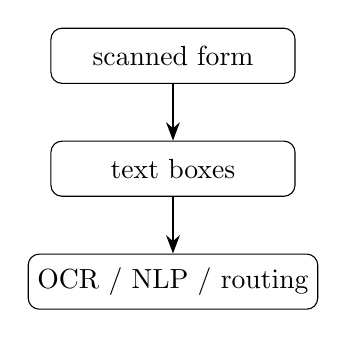
\begin{tikzpicture}[>=Stealth, node distance=0.72cm]
  \node[draw, rounded corners, fill=white, minimum width=3.1cm, minimum height=0.7cm] (a) {scanned form};
  \node[draw, rounded corners, fill=white, below=of a, minimum width=3.1cm, minimum height=0.7cm] (b) {text boxes};
  \node[draw, rounded corners, fill=white, below=of b, minimum width=3.1cm, minimum height=0.7cm] (c) {OCR / NLP / routing};
  \draw[->, thick] (a) -- (b);
  \draw[->, thick] (b) -- (c);
\end{tikzpicture}
\end{center}
\end{columns}
\end{frame}

% 3
\begin{frame}{Task: text blocks, not field semantics}
\begin{columns}[T]
\column{0.55\textwidth}
\begin{center}
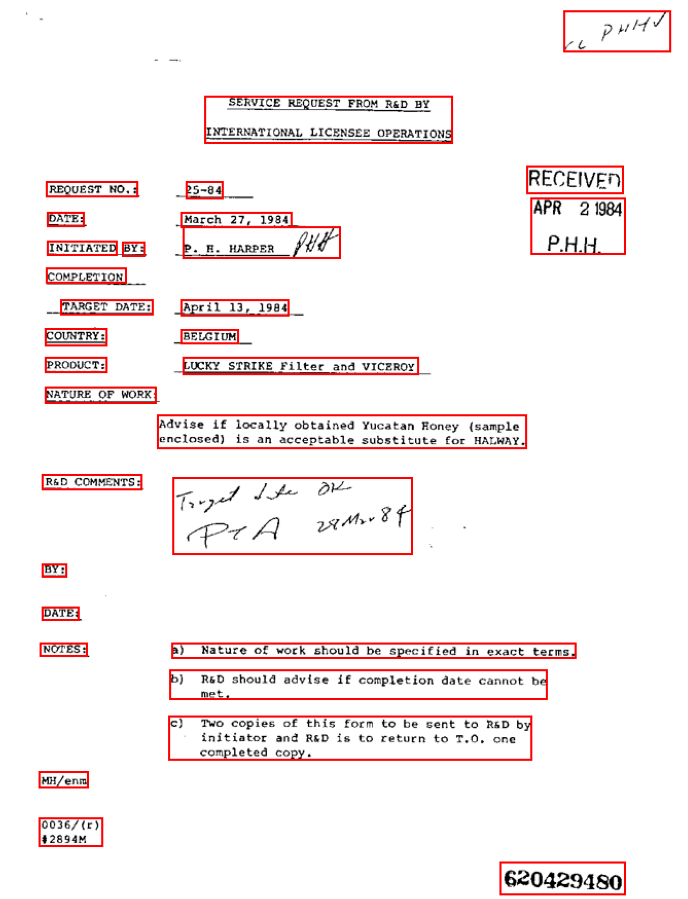
\includegraphics[height=4.9cm]{assets/Figure_2_qual.png}
\end{center}
\column{0.40\textwidth}
\textbf{Detection target}
\begin{itemize}
  \item one class: \texttt{text}
  \item one box per text segment
  \item no name, date or address class
\end{itemize}
\takeaway{This work is a preprocessing step for document understanding.}
\end{columns}
\end{frame}

% 4
\begin{frame}{Challenge: labels and domain gap}

\textbf{Limited labeled data}
\begin{itemize}
    \item Object detection requires bounding boxes for every text region.
    \item Creating and checking these annotations manually is time-consuming.
    \item This makes large labeled datasets expensive to create.
    %\item Large amounts of labeled real documents are therefore difficult to obtain.
\end{itemize}

\vspace{0.8em}

\textbf{Domain gap}
\begin{itemize}
    \item Synthetic documents can provide additional labeled training data.
    \item However, synthetic and real documents differ in text appearance, noise, text placement and other ways.
    \item A detector trained only on synthetic data may therefore generalize less well to real documents.
\end{itemize}

\vspace{0.8em}

%\textbf{Goal:} use synthetic data to reduce the need for manual labels, then use
%self-training to adapt the detector to real documents.

\end{frame}

% 5
\begin{frame}{Data: FUNSD}
\begin{columns}[T]
\column{0.55\textwidth}
\begin{center}
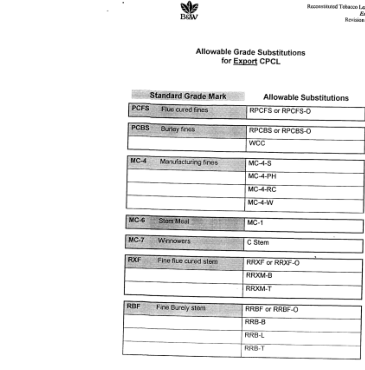
\includegraphics[height=5.1cm]{assets/real_form_tabular.png}
\end{center}
\column{0.40\textwidth}
\textbf{FUNSD}
\begin{itemize}
  \item 199 fully annotated scanned business forms
  \item 149 training forms, 50 test forms
  \item grayscale / black and white
  \item varying scan quality and resolution
\end{itemize}
\vspace{0.35em}
\textbf{Used here}
\begin{itemize}
  \item synthetic pages are generated from training layouts
  \item final evaluation stays on real test forms
\end{itemize}
\end{columns}
\end{frame}

% 6
\begin{frame}{Synthetic data generation}
\begin{center}
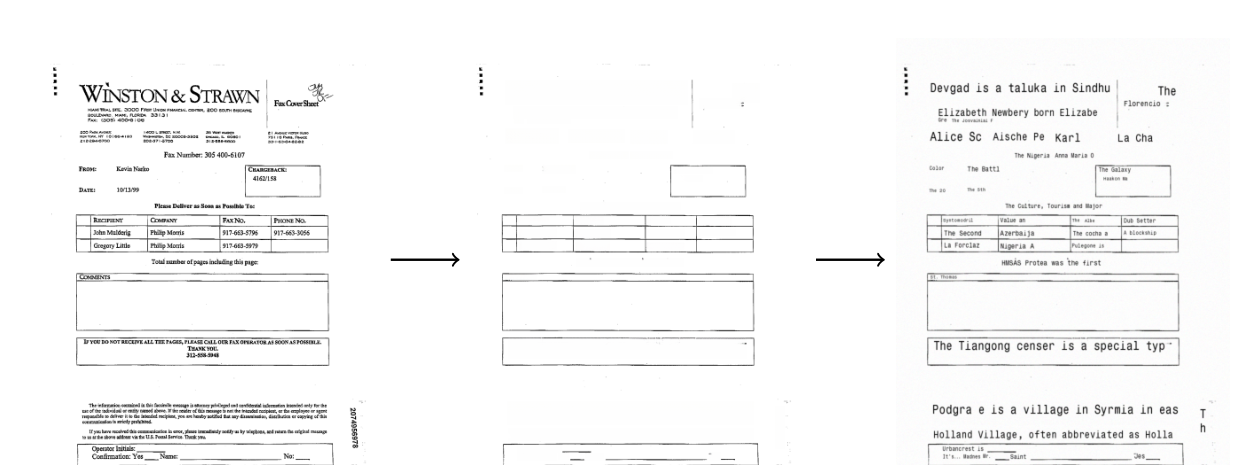
\includegraphics[width=0.94\linewidth]{assets/pipeline_crop.png}
\end{center}

\begin{itemize}
  \item Existing annotations mark the original text regions.
  \item Inpainting removes the original text and reconstructs the background.
  \item This keeps the document layout and non-text structure largely intact.
  \item New Wikipedia text is inserted and the resulting location boxes are stored.
  %\item Bounding-box masks guide Inpaint Anything with LaMa to remove the original text and reconstruct the background from the surrounding image context.
\end{itemize}
\end{frame}

% 7
\begin{frame}{Detector: Faster R-CNN}

\begin{columns}[T]

\column{0.43\textwidth}
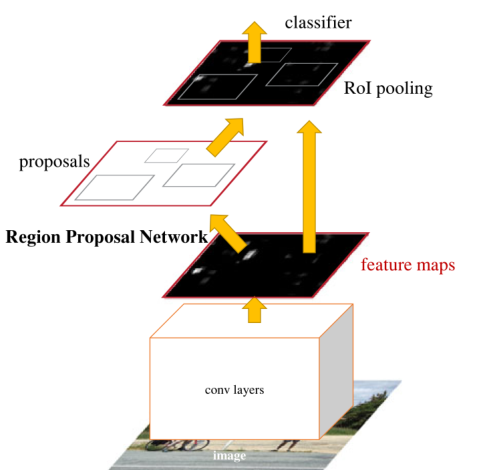
\includegraphics[width=0.98\linewidth]{assets/frcnn_crop.png}
\shortnote{Figure adapted from Ren et al.}

\column{0.52\textwidth}

\begin{enumerate}
  \item \textbf{Feature extraction}\\
  ResNet-50 extracts image features; FPN provides multiple scales.

  \item \textbf{Region proposals}\\
  The RPN proposes candidate regions likely to contain text.

  \item \textbf{RoI features}\\
  Features for each proposal are converted to a fixed-size representation.

  \item \textbf{Classification and refinement}\\
  Proposals are classified as text or background and their boxes are refined.

  \item \textbf{Final detections}\\
  Overlapping predictions are filtered to produce the final text boxes.
\end{enumerate}

\end{columns}
\end{frame}

% 8
\begin{frame}{Evaluation}

\begin{center}
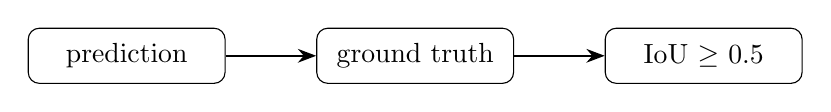
\begin{tikzpicture}[>=Stealth, node distance=1.15cm]
  \node[draw, rounded corners, fill=white, minimum width=2.5cm, minimum height=0.7cm] (p) {prediction};
  \node[draw, rounded corners, fill=white, right=of p, minimum width=2.5cm, minimum height=0.7cm] (g) {ground truth};
  \node[draw, rounded corners, fill=white, right=of g, minimum width=2.5cm, minimum height=0.7cm] (m) {IoU $\geq$ 0.5};
  \draw[->, thick] (p) -- (g);
  \draw[->, thick] (g) -- (m);
\end{tikzpicture}
\end{center}

\vspace{0.35em}

\begin{center}
\EvaluationTable
\end{center}

\vspace{0.35em}

\begin{center}
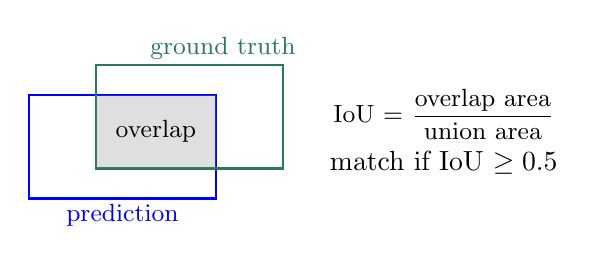
\begin{tikzpicture}[scale=0.85]
  % boxes
  \draw[thick, blue] (0,0) rectangle (2.8,1.55);
  \draw[thick, greenaccent] (1.0,0.45) rectangle (3.8,2.0);

  % overlap
  \fill[gray, opacity=0.25] (1.0,0.45) rectangle (2.8,1.55);

  % labels
  \node[blue] at (1.4,-0.25) {\small prediction};
  \node[greenaccent] at (2.9,2.25) {\small ground truth};
  \node at (1.9,1.0) {\small overlap};

  % formula
  \node[align=center] at (6.2,1.0) {\small
    IoU $=$ $\dfrac{\text{overlap area}}{\text{union area}}$\\[0.3em]
    match if IoU $\geq 0.5$
  };
\end{tikzpicture}
\end{center}

\end{frame}

% 9
\begin{frame}{Self-training: teacher and student}
\begin{center}
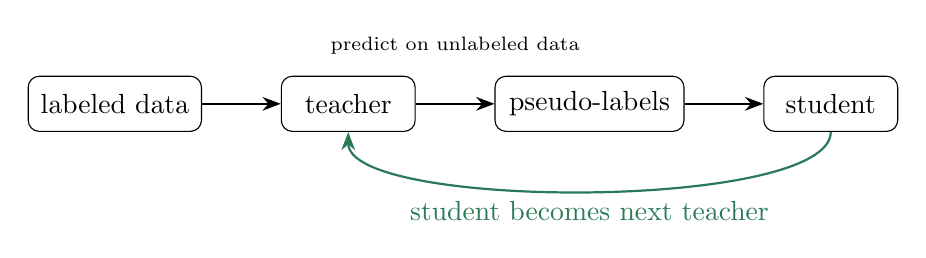
\begin{tikzpicture}[>=Stealth, node distance=1.0cm]
  \node[draw, rounded corners, fill=white, minimum width=2.2cm, minimum height=0.7cm] (a) {labeled data};
  \node[draw, rounded corners, fill=white, right=of a, minimum width=1.7cm, minimum height=0.7cm] (b) {teacher};
  \node[draw, rounded corners, fill=white, right=of b, minimum width=2.4cm, minimum height=0.7cm] (c) {pseudo-labels};
  \node[draw, rounded corners, fill=white, right=of c, minimum width=1.7cm, minimum height=0.7cm] (d) {student};
  \draw[->, thick] (a) -- (b);
  \draw[->, thick] (b) -- node[above=0.5, font=\scriptsize]{predict on unlabeled data} (c);
  \draw[->, thick] (c) -- (d);
  \draw[->, thick, greenaccent] (d.south) .. controls +(0,-1.0) and +(0,-1.0) .. node[below]{student becomes next teacher} (b.south);
\end{tikzpicture}
\end{center}

\vspace{0.65em}

\begin{itemize}
  \item A teacher is trained from trusted labeled data.
  \item Confident predictions on unlabeled data are treated as temporary training labels.
  \item student trains on synthetic pages with ground-truth boxes and pseudo-labeled real pages
  \item \textbf{Goal:} use unlabeled real data to improve the model automatically.
\end{itemize}

\end{frame}

% 10
\begin{frame}{ASTOD-inspired loop}
\begin{columns}[T]
\column{0.60\textwidth}
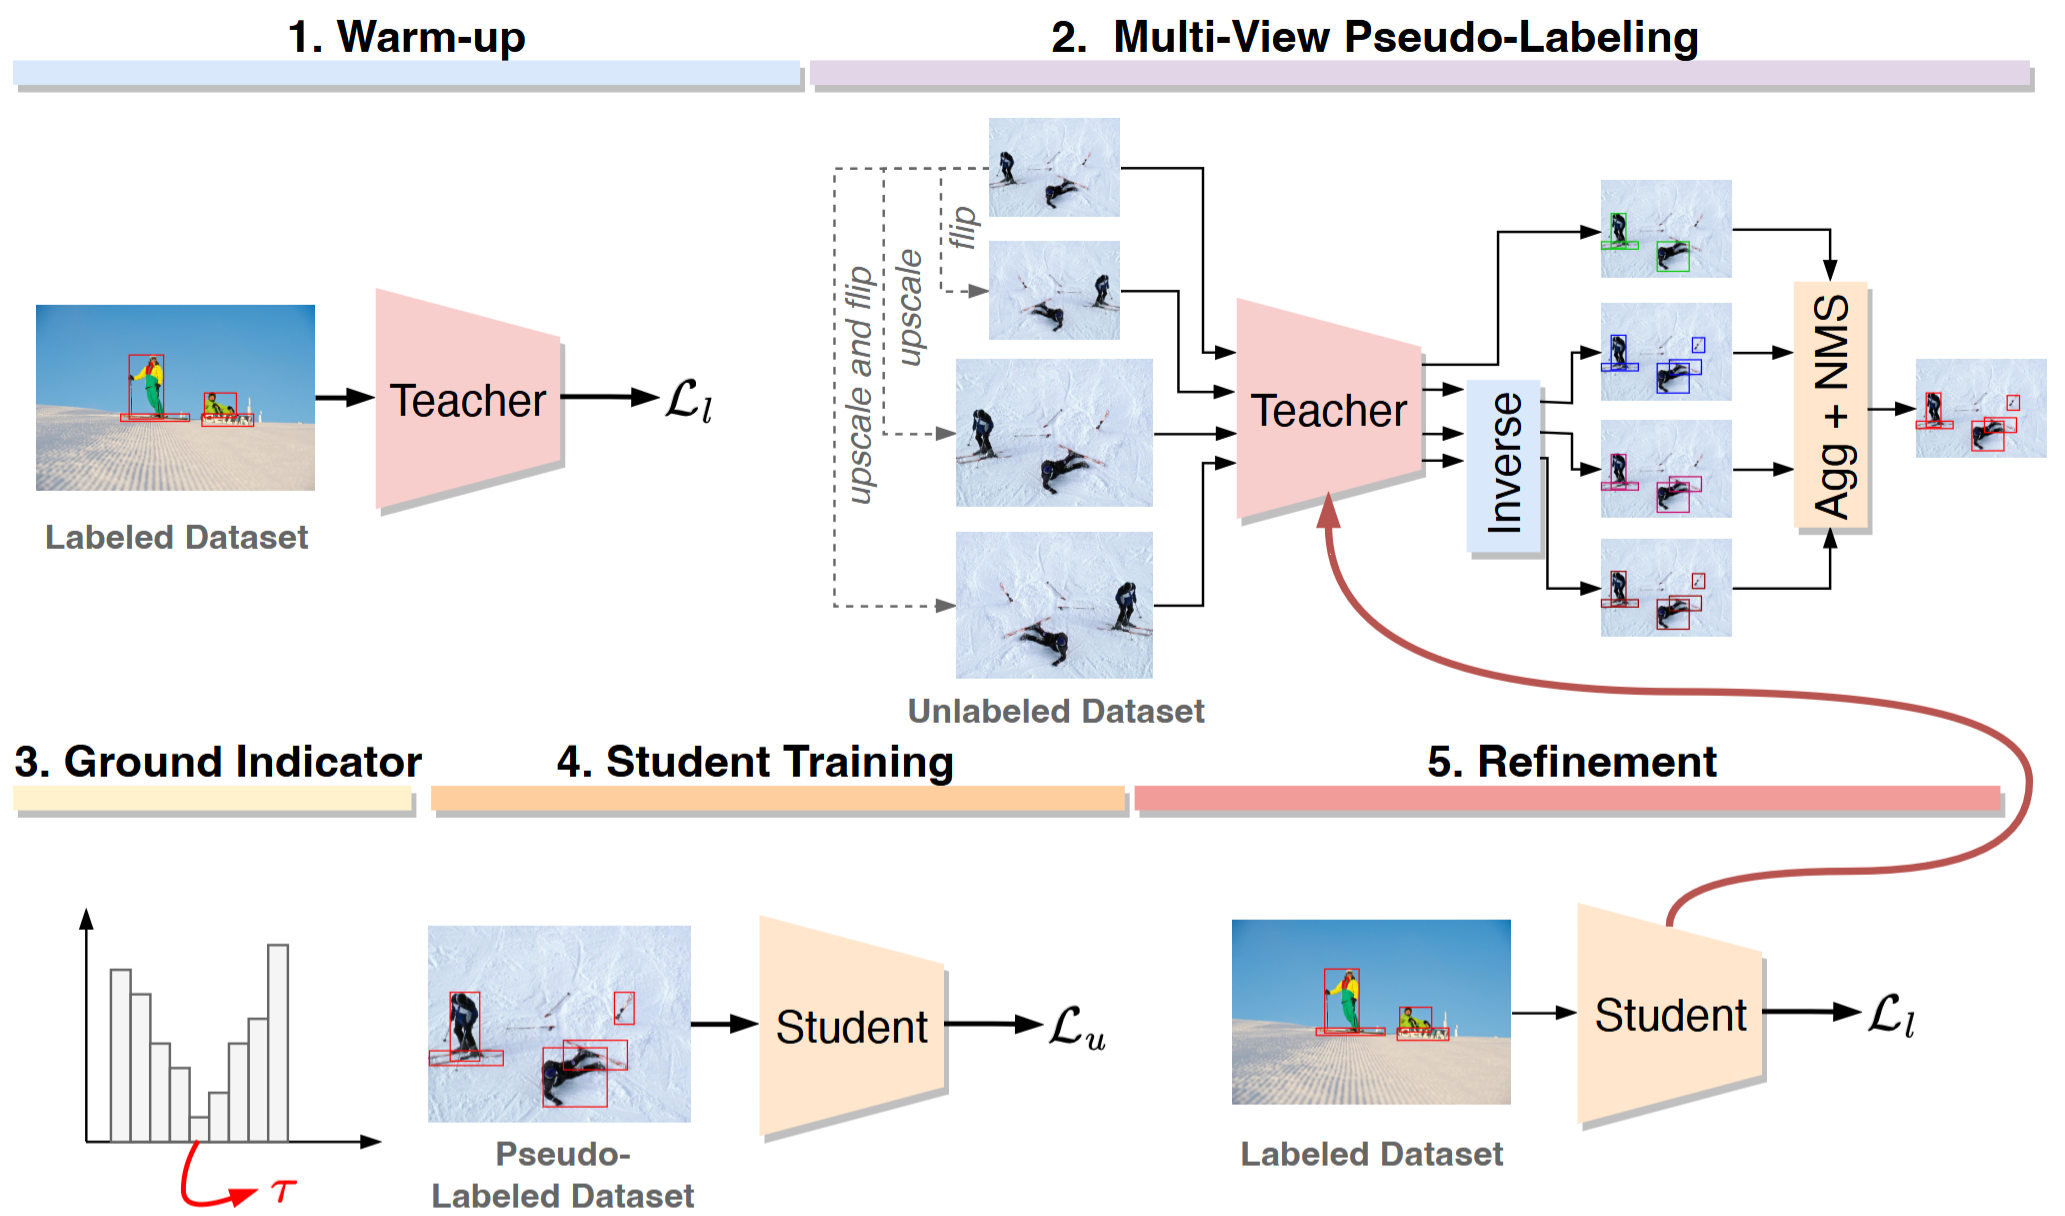
\includegraphics[width=\linewidth]{assets/Selftraining Full-steps.png}
\column{0.36\textwidth}
\begin{itemize}
  \item warm-up on synthetic pages
  \item teacher predicts boxes on real pages
  \item histogram threshold filters predictions
  \item student trains on synthetic labels and teacher-labeled real pages
\end{itemize}
\vspace{0.3em}
\iffalse
\textbf{Adaptation in this thesis}
Trusted synthetic labels remain in every round
to limit pseudo-label drift.
\fi
\end{columns}
\shortnote{ASTOD reference: Vandeghen et al., ICCV Workshops 2023.}
\end{frame}

% 11
\begin{frame}{Experimental setup}
\begin{center}
\SetupTable
\end{center}
\takeaway{The same detector, evaluation rule and data flow are used for the main comparisons.}
\end{frame}

% 12
\begin{frame}{Parameter choice}
\experimentquestion{Choose one stable optimizer setting before comparing the main experiments.}
\begin{columns}[T]
\column{0.48\textwidth}
\textbf{Literature starting point}
\begin{itemize}
  \item FUNSD evaluates Faster R-CNN as a text-detection baseline.
  \item Original Faster R-CNN training uses SGD, momentum 0.9 and weight decay 0.0005.
  \item ASTOD uses Faster R-CNN with FPN and a ResNet-50 backbone for teacher-student training.
\end{itemize}
\column{0.48\textwidth}
\textbf{Fixed setting in this thesis}
\begin{center}
\begin{tabular}{lc}
\toprule
Parameter & Value \\
\midrule
%Optimizer & SGD \\
Learning rate & 0.006 \\
Momentum & 0.8 \\
Weight decay & 0.0005 \\
\bottomrule
\end{tabular}
\end{center}
\vspace{0.35em}
\small Exact values were selected by preliminary sweeps on this setup, then kept fixed.
\end{columns}
%\shortnote{References: Ren et al., Faster R-CNN, 2017; Jaume et al., FUNSD, 2019; Vandeghen et al., ASTOD, 2023.}
\end{frame}

% 13
\begin{frame}{Baselines}
\experimentquestion{How large is the gap before using self-training?}
\begin{center}
\BaselineTable
\end{center}
\vspace{0.35em}
\begin{center}
The synthetic-only model is about 10 F1 points below training with real labels.
\end{center}
\vspace{0.4em}

\end{frame}


%14
\begin{frame}{Synthetic variants}
\begin{columns}[T]
\column{0.49\textwidth}
\begin{center}
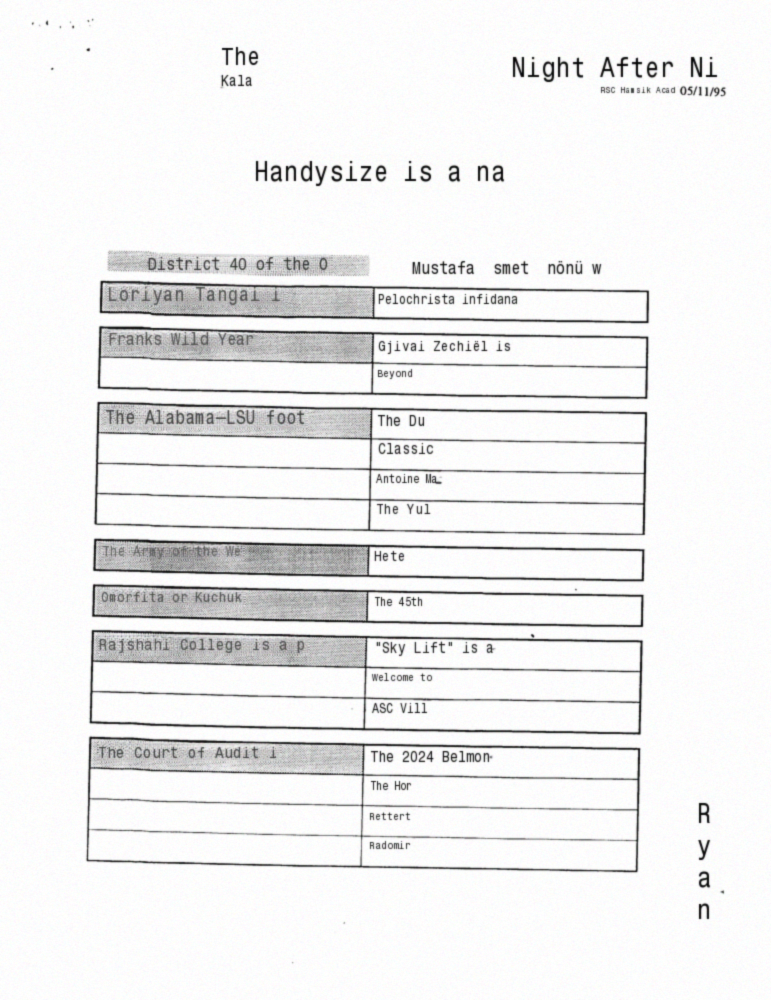
\includegraphics[height=5.9cm]{assets/inpainted_example.png}
\end{center}
\centering\textbf{Inpainting}\par
{\scriptsize Original text is removed. The surrounding scan background is preserved.}
\column{0.49\textwidth}
\begin{center}
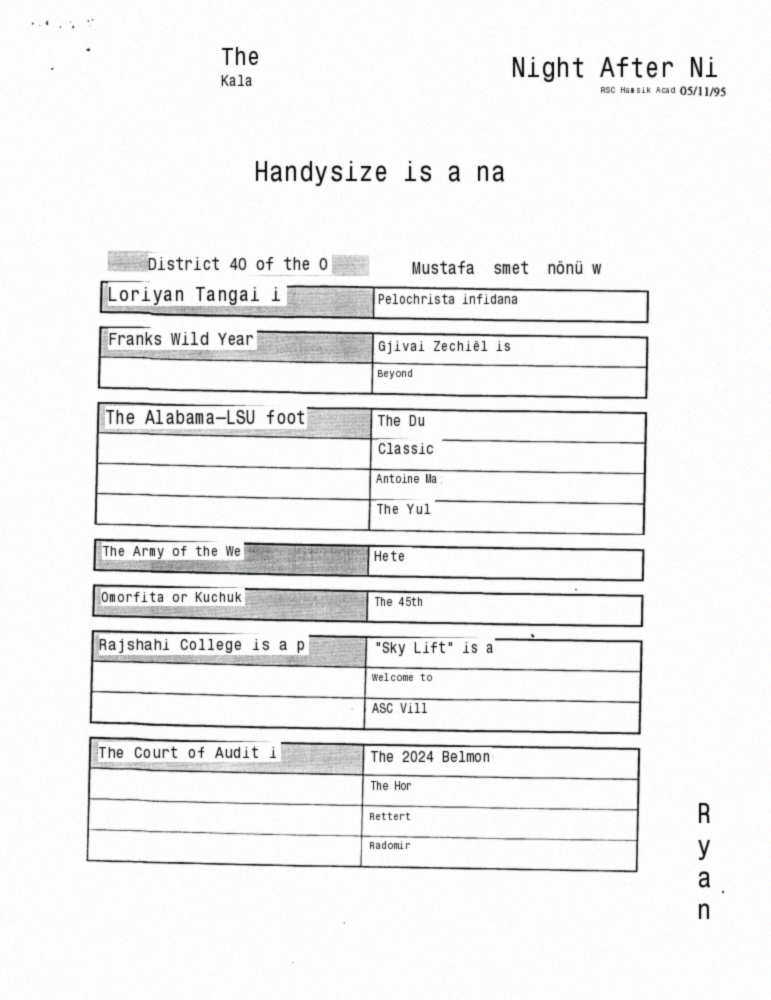
\includegraphics[height=5.9cm]{assets/white_example.png}
\end{center}
\centering\textbf{White background}\par
{\scriptsize Original text regions are replaced with white rectangles before inserting text.}
\end{columns}
\end{frame}

% 15
\begin{frame}{Synthetic method comparison}
\experimentquestion{Does preserving the scan background improve transfer to real forms?}
\begin{center}
\GenerationTable
\end{center}
\vspace{0.55em}
\begin{center}
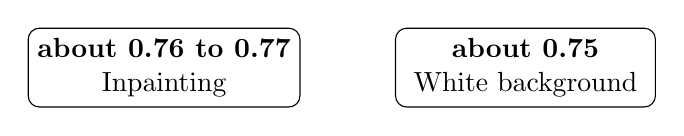
\begin{tikzpicture}[node distance=1.2cm]
  \node[draw, rounded corners, fill=white, align=center, minimum width=3.3cm, minimum height=1.0cm] (a) {\textbf{about 0.76 to 0.77}\\Inpainting};
  \node[draw, rounded corners, fill=white, align=center, minimum width=3.3cm, minimum height=1.0cm, right=of a] (b) {\textbf{about 0.75}\\White background};
\end{tikzpicture}
\end{center}
\takeaway{Inpainting has a small advantage in the stronger comparison.}
\end{frame}

%16
\begin{frame}{Amount of synthetic data}
\experimentquestion{How much synthetic data is needed for useful self-training?}
\begin{center}
\SyntheticAmountTable
\end{center}
\vspace{0.45em}
\textbf{Result:} reduced subsets still work, while the full long-run setting reaches the strongest result.
\end{frame}


% 17
\begin{frame}{Main result: self-training over 100 iterations}
\experimentquestion{How does performance change as teacher-student iterations continue?}
\begin{center}
\begin{tikzpicture}
  \node[inner sep=0] (img) {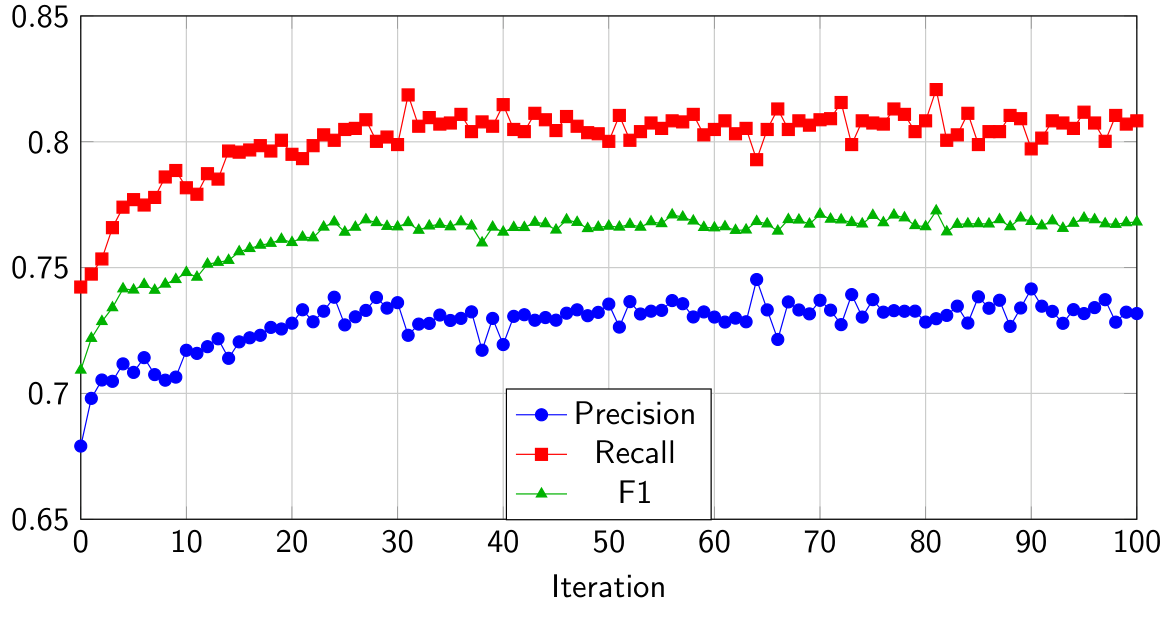
\includegraphics[width=0.88\linewidth]{assets/selftraining100_fullchart.png}};
  \node[draw=greenaccent, rounded corners, fill=white, text=navy, font=\bfseries\scriptsize] at ($(img.south east)+(-1.9cm,2.45cm)$) {F1 $\approx$ 0.77};
\end{tikzpicture}
\end{center}
\vspace{-0.15em}
\begin{center}\small F1 rises from about 0.70 to about 0.77. Most of the gain appears in the first 20 iterations.\end{center}
\end{frame}



% 18
\begin{frame}{Keep trusted synthetic labels}

\experimentquestion{Does keeping synthetic training data stabilize self-training?             }
\vspace{0.35em}
\small
%\textbf{Important:} The synthetic pages and their ground-truth bounding boxes remain in the training set in every self-training round.
\begin{center}
\AnchorTable
\end{center}



\vspace{0.25em}
\small
\textbf{Pseudo-labeled real pages} are real images whose training boxes were generated by the teacher model.

\vspace{0.45em}
\begin{center}
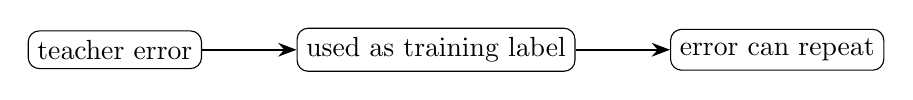
\begin{tikzpicture}[>=Stealth, node distance=1.2cm]
  \node[draw, rounded corners, fill=white] (e) {teacher error};
  \node[draw, rounded corners, fill=white, right=of e] (l) {used as training label};
  \node[draw, rounded corners, fill=white, right=of l] (d) {error can repeat};
  \draw[->, thick] (e) -- (l);
  \draw[->, thick] (l) -- (d);
\end{tikzpicture}
\end{center}

\takeaway{Keeping trusted synthetic data stabilizes self-training against repeated pseudo-label errors.}

\end{frame}

% 19
\begin{frame}{Real-label experiments}
\experimentquestion{Is self-training still useful when the starting model already has real supervision?}
\begin{center}
    
\begin{tabular}{lc}
\toprule
Experiment & F1 \\
\midrule
Real-only baseline & 0.801 \\
Real-start self-training & 0.806 \\
Real + synthetic self-training & 0.814 \\
\bottomrule
\end{tabular}
\end{center}
\takeaway{Self-training gives smaller gains when the supervised starting model is already strong.}

\end{frame}

% 20
\begin{frame}{Main findings}
\begin{enumerate}
  \item Synthetic pages are a useful starting point: about 0.70 F1.
  \item Self-training raises the result to about 0.77 F1.
  \item Keeping trusted synthetic data stabilizes self-training against repeated pseudo-label errors.
  \item Inpainting is slightly stronger than the white-background variant in the stronger comparison.
\end{enumerate}
\takeaway{Real labels remain strongest, but self-training closes much of the gap.}
\end{frame}

% 21
\begin{frame}{Limitations}
\begin{itemize}
  \item Main evaluation on one form dataset.
  \item One detection class: \texttt{text}.
  \item Synthetic pages still have limited font and handwriting variation.
  \item Results were not averaged over many independent random seeds.
  \item Pseudo-label quality depends on the current teacher model.
  \item The synthetic data still reuses layouts from annotated source forms.
\end{itemize}
\end{frame}

% 22
\begin{frame}{Conclusion and outlook}

\textbf{Conclusion}
\begin{itemize}
  \item Synthetic forms are a useful starting point for text-block detection.
  \item Self-training reduces much of the gap to real-label training.
  \item Real supervision still performs best.
\end{itemize}

\vspace{0.5em}

\textbf{Outlook}
\begin{itemize}
  \item More realistic synthetic data, including fonts and handwriting.
  \item Evaluation on additional datasets and newer detectors.
\end{itemize}

\vfill
\begin{center}\Large\bfseries Thank you for listening.\end{center}
\end{frame}

\iffalse
% 23 backup
\begin{frame}{Backup: implementation details}
\begin{center}
\ImplementationTable
\end{center}
\end{frame}

% 24 backup
\begin{frame}{Backup: key numbers}
\begin{center}
\KeyNumbersTable
\end{center}
\end{frame}

% 25 backup
\begin{frame}{Backup: parameter sweeps}
\begin{columns}[T]
\column{0.33\textwidth}
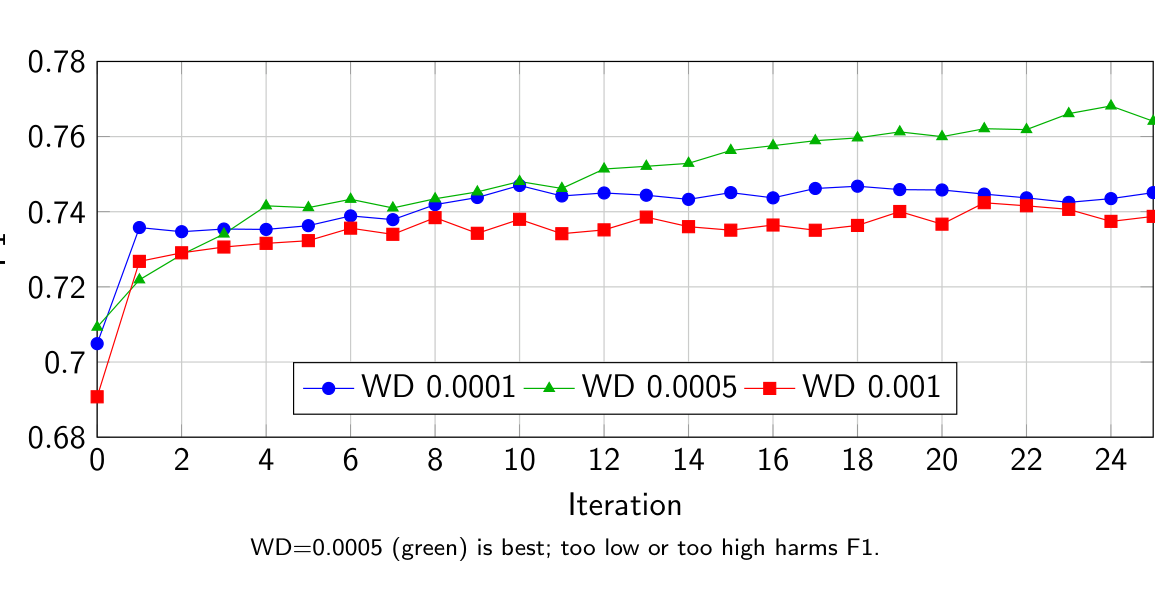
\includegraphics[width=\linewidth]{assets/wd_crop.png}
\centering\scriptsize Weight decay
\column{0.33\textwidth}
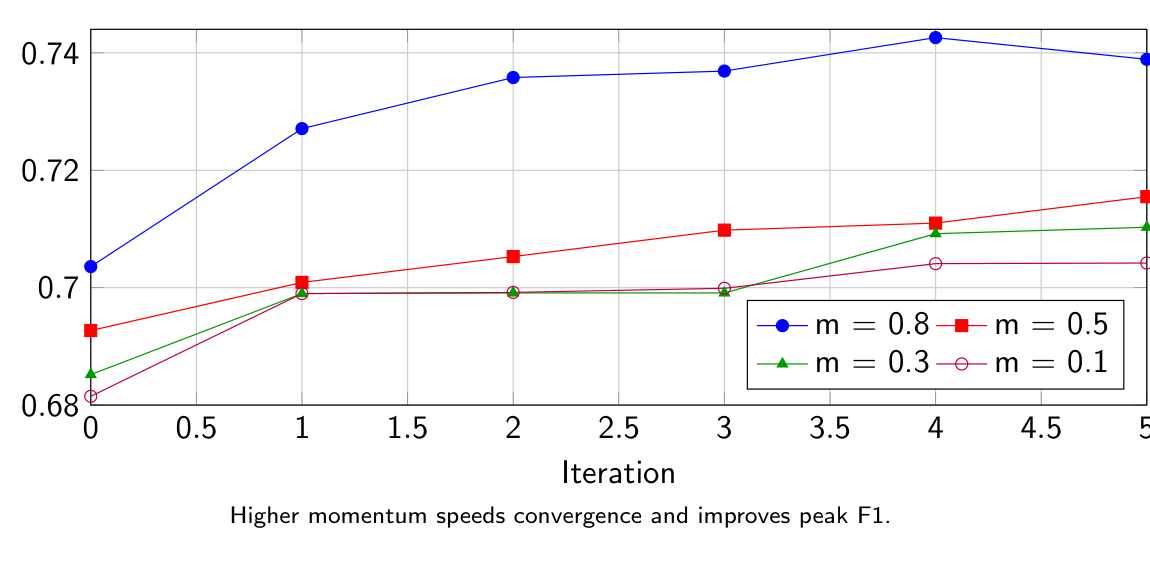
\includegraphics[width=\linewidth]{assets/momentum_crop.png}
\centering\scriptsize Momentum
\column{0.33\textwidth}
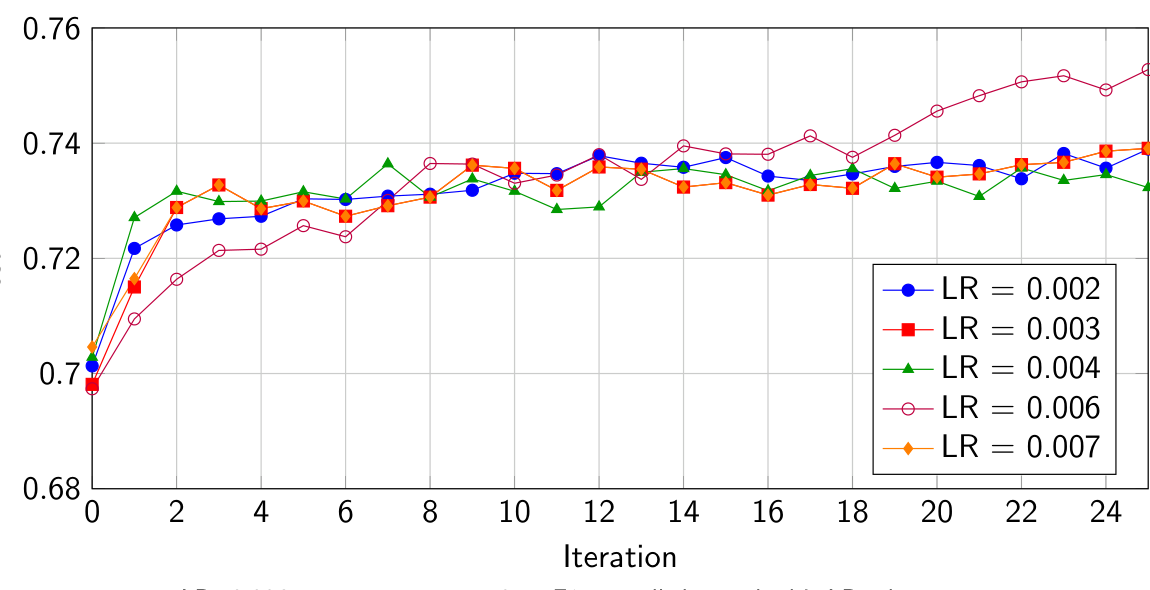
\includegraphics[width=\linewidth]{assets/lr_crop.png}
\centering\scriptsize Learning rate
\end{columns}
\vspace{0.45em}
\small These preliminary sweeps selected the values used on slide 12. They are shown here only if the parameter choice is questioned.
\end{frame}
\fi
\end{document}
